%databaseimpl.tex
The implementation of the MySQL database is done in MySQL Workbench 5.2.40.

Due to the dependencies of the various tables, the order of how they need to be created is quite strict, see \autoref{MySQLcode}. 
To make sure the \code{username} and \code{userID} attributes follows the previously stated constraints, they have been made \code{UNIQUE NOT NULL} and \code{userID} furthermore has \code{AUTO_INCREMENT} as seen in \autoref{createAuthUsers}. 
This makes sure there can be no one with the same user-name or user ID, and furthermore \code{userID} will automatically increase when new data is inserted. 
This also guarantees a one-to-one relation between both \code{Profile} and \code{AuthUsers}, as well as \code{Departments} and \code{AuthUsers}. 

To distinguish departments and profiles a attribute called \code{aRole} is used. 
This is an integer and will hold a number, which will be used at software level. The same applies for \code{Profile}'s attribute \code{pRole}, see \autoref{createProfile}.

The MySQL Workbench provides the functionality to create an ER diagram from an existing database, this diagram is shown in \autoref{fig:workbenchRight}. The diagram is not completely as MySQL workbench creates it, the real is shown in the appendix \autoref{errDiagram}. But this is a error in the software, as seen in \autoref{fig:workbenchWrong}, the tool generates the \code{Profiles}$\rightarrow$\code{AuthUsers} as a one-to-many relation. However, this is not possible since the \code{idUser} attribute in \code{AuthUsers} is unique, as seen in \autoref{createAuthUsers}, the same goes for both \code{Departments} and \code{Medias}.

\begin{figure}
	\centering
		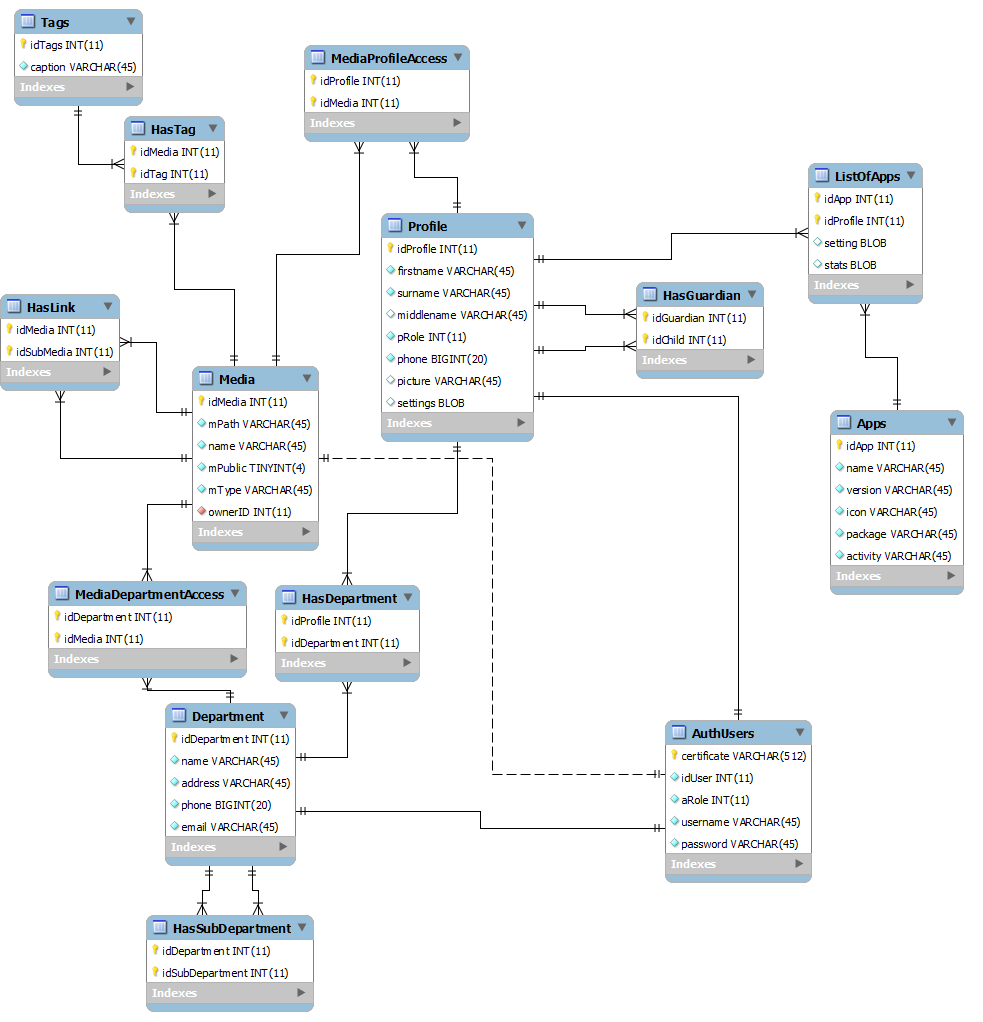
\includegraphics[width=1.00\textwidth]{images/workbenchRight.png}
	\caption{The ER diagram}
	\label{fig:workbenchRight}
\end{figure}

To make the deletion of data easy, many of the attributes in the tables has the constraint \code{ON DELETE CASCADE}. This can be dangerous, as side-effects can result in unintended data being deleted. To avoid this, the software level implementation needs to warn the user when deleting data. Furthermore an analysis has been made to argue which attributes can have this constraint. The following tables and attributes have the cascade constraint: 
\begin{verbatim}
``Profiles''.''idProfile'', 
``ListOfApps''.''idProfile'', 
``HasDepartment''.''idProfile'', 
``HasGuardian''.''idGuardian'', 
``HasGuardian''.''idChild'', 
``Media''.''OwnerID'', 
``HasTag''.''idMedia'', 
``HasLink''.''idMedia'', 
``HasLink''.''idSubMedia'',
''MediaProfileAccess''.''idProfile''.
\end{verbatim}

\subsubsection*{Use case}
 A use case of the constraint is:
\begin{quotation}
``A user ``Jesper'' wishes to delete his entire profile''
\end{quotation}
What will happen is:
\begin{enumerate}
	\item A deletion of the ``userID'' in ``AuthUsers'' is executed
	\item The relation between ``AuthUsers'' and ``Profiles'' will delete the profile
	\item The relation between ``Profiles'' and ``HasGuardian'' will delete all fields where the ``userID'' is either ``idGuardian'' or ``idChild''
	\item The relation between ``AuthUsers'' and ``Media'' will delete all fields where ``idUser'' is the owner
	\item The relation between ``Media'' and ``HasTag'' will delete all fields where ``HasTags''.``idMedia'' equals ``idMedia''
	\item The relation between ``Media'' and ``HasLink'' will delete all fields where ``HasLink''.''idMedia'' or ``HasLink''.''idSubMedia'' equals ``idMedia''
\end{enumerate}

